%% Slide 18.
\begin{frame}
\begin{itemize}[<+->]
\item
Highly interactive virtual reality systems such as massively multiplayer
online games (MMOGs) necessitates highly robust and efficient architectures.
\item
Distributed implementations must deal with challenges such as: supporting very
large numbers of users, the need to maintain robustness, balancing the
processing load, reducing user latency, and minimizing thrashing effects.
There are no unified methods that attack these problems cohesively.
\item
The next paper presents a software design intended for distributed high
performance computing facilities in
which the world is divided into a regular lattice of overlapping
cells (providing redundancy), which are dynamically assigned to
servers within the High Performance Computing.
\end{itemize}
\end{frame}

\subsection{Requirements}

%% Slide 19.
\begin{frame}
\frametitle{Requirements for Large-scale, Distribuited System}
\framesubtitle{}
\begin{block}{Robustness to Hardware Failure}
Distributed systems
should avoid single-point-of-failure problems where part of the
world state is lost with a server failure.
\end{block}
\pause
\begin{block}{Balancing of Processing Load}
Dynamic entity behaviors
demand responsive methods for shifting processor load to
conserve computational resources.
\end{block}
\pause
\begin{block}{Mitigation of Thrashing}
Distributed systems should avoid
repeated inefficient transitions of objects between resources.
\end{block}
\pause
\begin{block}{Reduction of User Latency}
Game systems must avoid
unacceptable latencies between the user clients and the servers.
\end{block}
\end{frame}

%% Slide 19.
\begin{frame}
\frametitle{Related Work}
\framesubtitle{}
Distributed MMOGs and other multi-server, large-scale VR
systems use a variety of methods to address the four desired
capabilities mentioned above.
\begin{itemize}
\item<2->
Sharding method.
\item<3->
Zoning methods.
\item<4->
Peer-to-Peer (P2P) paradigm.
\end{itemize}
\end{frame}

\subsection{An Overlapping Zone-Based Architecture}

%% Slide 20.
\begin{frame}[fragile]
\frametitle{An Overlapping Zone-Based Architecture}
\framesubtitle{}
\begin{itemize}
\item<1->
The virtual world is divided into a lattice of small, \alert{overlapping
cells} (zones).
\item<2->
Cells must completely tessellate the region of interest.
\item<3->
The cell overlap provides a mechanism for redundancy to protect against server
crash, it facilitates a system for seamless migration across cell
boundaries, and it allows load balancing methods.
\item<4->
Cells are pre-distributed amongst the servers for processing.
\item<5->
Entity (object and user data in
the environment) are assigned to a cell based on the location of
the object in the world, and the server managing that cell can be
considered the \alert{master host} of such objects.
\end{itemize}
\end{frame}

%% Slide 21.
\begin{frame}[fragile]
\frametitle{An Overlapping Zone-Based Architecture}
\framesubtitle{Loose Cell Overlap Pattern}
\begin{columns}

\begin{column}{0.5\textwidth}
\begin{block}{The master-slave relationship is determinated by the overlap.}
Server 1 (Layer 1) is master to object Q and slave to object R.
Server 2 (Layer 2) is master to object R and slave to object Q.
\end{block}
\begin{block}{}<2->
Each cell is divided into four quadrants: $(1,1); (1,2); (2,1); (2,2)$.
\end{block}
\end{column}

\begin{column}{0.5\textwidth}
\begin{center}
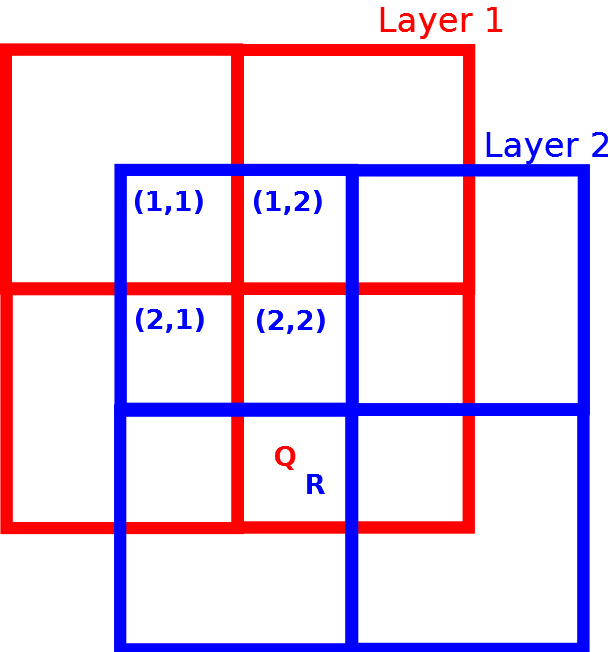
\includegraphics[scale=.80]{celloverlap.png}
\end{center}
\end{column}

\end{columns}
\end{frame}


%% Slide 22.
\begin{frame}[fragile]
\frametitle{An Overlapping Zone-Based Architecture}
\framesubtitle{Update Responsibilities \& Area of Interest}
\begin{columns}

\begin{column}{0.65\textwidth}
Update responsibilities of entities are transferred between
servers as those entities are repositioned throughout the world.

\begin{block}{}<2->
Such decisions are made by using defined check-in and check-out boundaries for
entities moving between cells.
\end{block}

\begin{block}{Area of Interest}<3->
Area of Interest (AoI) is defined around an entity, and when that AoI
intersects the boundary, management of the entity is shifted.
\end{block}
\end{column}

\begin{column}{0.35\textwidth}
\begin{center}
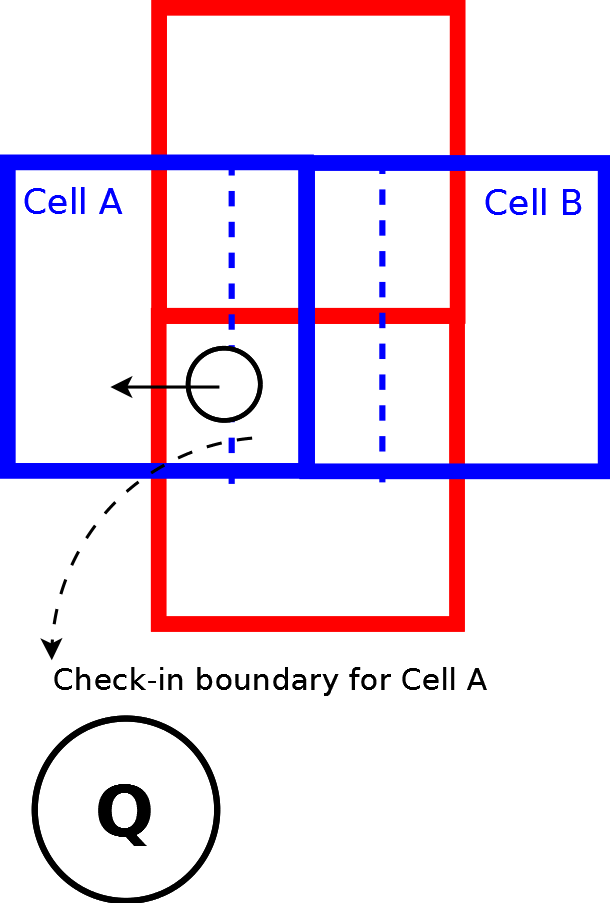
\includegraphics[scale=.80]{aoi.png}
\end{center}
\end{column}

\end{columns}
\end{frame}

\subsection{Analysis}

%% Slide 23.
\begin{frame}[fragile]
\frametitle{Analysis}
\framesubtitle{Entity Motion}
\begin{center}
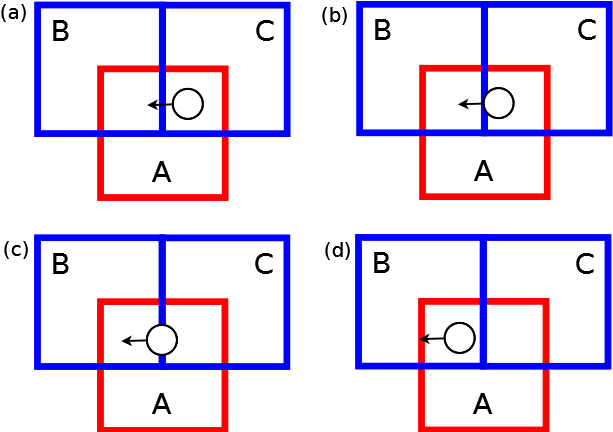
\includegraphics[scale=.80]{motion.png}
\end{center}
\end{frame}

%% Slide 24.
\begin{frame}[fragile]
\frametitle{Analysis}
\framesubtitle{Entity Motion}
\begin{center}
\begin{table}
\caption{Favorable Server-Motion allocation for Cost minimization.}
\begin{tabular}{|c|c|}
\hline
\parbox[t]{4cm}{For direction of motion of entity} &
\parbox[t]{4cm}{Master server of entity should be that
which is the master of the cell that hold the entity} \\
\hline
$\longrightarrow\quad$ $\downarrow\quad$ $\searrow\quad$ & (1,1) \\
\hline
$\longleftarrow\quad$ $\downarrow\quad$ $\swarrow\quad$ & (1,2) \\
\hline
$\longrightarrow\quad$ $\uparrow\quad$ $\nearrow\quad$ & (2,1) \\
\hline
$\longleftarrow\quad$ $\uparrow\quad$ $\nwarrow\quad$ & (2,2) \\
\hline
\end{tabular}
\end{table}
\end{center}
\end{frame}

%% Slide 25.
\begin{frame}[fragile]
\frametitle{Analysis}
\framesubtitle{Server Crash \& Dynamic Allocation}
\begin{block}{Server Crash}
\begin{itemize}
\item <2->
A natural fault tolerance is accomplished in this design because
of the redundancy provided by overlapping cells.
\item <3->
When a server crashes, any entities over which it had master control are
already replicated on at least one other server.
\item <4->
The system must merely transfer master control and needn't seekk data from a
crashed machine.
\end{itemize}
\end{block}
\begin{block}{Dynamic Cell Allocation}<5->
Dynamic cell allocation methods between servers must
accomplish a multitude of things with reasonable efficiency.
\end{block}
\end{frame}

%% Slide 26.
\section*{References}
\begin{frame}
\frametitle{References}
\begin{thebibliography}{}
\bibitem{van} S.A. van Houten, P.H.M. Jacobs, \emph{An Architecture for
Distribuited Simulation Games},
Proceedings of the 2004 \emph{Winter Simulation Conference};
\bibitem{zyda} M. Zyda, \emph{From Visual Simulation to Virtual Reality to
Games}, IEE Computer Society, September 2005;
\bibitem{ghosh} C. Ghosh, R.P. Wiegand, B. Goldiez, T.Dere, \emph{An
Architecture Supporting Large Scale MMOGs},
Proceedings of the 3rd International ICST Conference on Simulation Tools
and Technique.
\end{thebibliography}
\end{frame}
